\begin{figure}[H]
\centering
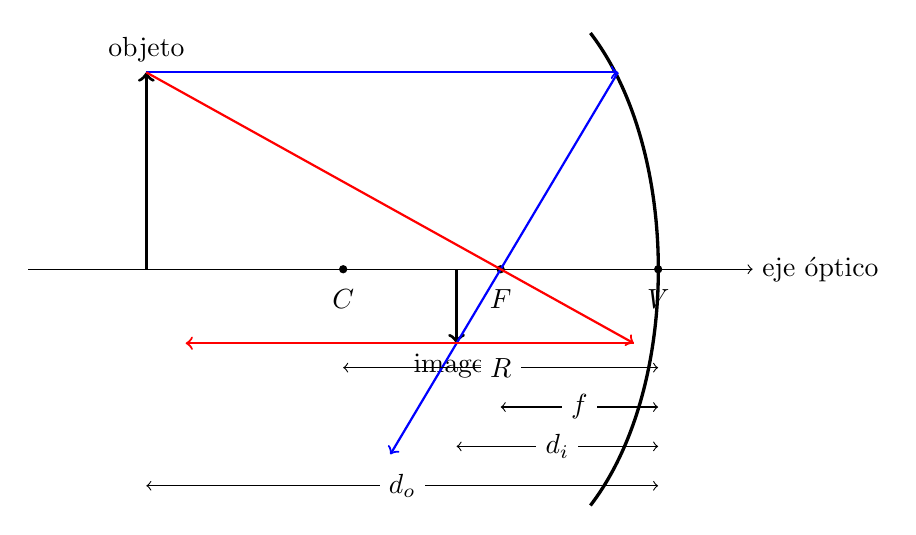
\begin{tikzpicture}[scale=1.0]
  \draw[->] (-8,0) -- (1.2,0) node[right] {eje óptico};
  \draw[very thick] (-0.86,-3) .. controls (0.29,-1.5) and (0.29,1.5) .. (-0.86,3);
  \foreach \x/\lab in {0/V,-2/F,-4/C}{
    \fill (\x,0) circle (1.5pt) node[below=4pt] {$\lab$};
  }
  \draw[->,very thick] (-6.5,0) -- (-6.5,2.5) node[above] {objeto};
  \draw[->,very thick] (-2.56,0) -- (-2.56,-0.94) node[below] {imagen};
  \draw[->,blue,thick] (-6.5,2.5) -- (-0.51,2.5);
  \draw[->,blue,thick] (-0.51,2.5) -- (-3.4,-2.35);
  \draw[->,red,thick] (-6.5,2.5) -- (-2,0) -- (-0.31,-0.94);
  \draw[->,red,thick] (-0.31,-0.94) -- (-6.0,-0.94);
  \draw[<->] (-6.5,-2.75) -- (0,-2.75) node[midway,fill=white] {$d_o$};
  \draw[<->] (-2.56,-2.25) -- (0,-2.25) node[midway,fill=white] {$d_i$};
  \draw[<->] (-2,-1.75) -- (0,-1.75) node[midway,fill=white] {$f$};
  \draw[<->] (-4,-1.25) -- (0,-1.25) node[midway,fill=white] {$R$};
\end{tikzpicture}
\caption{Formación de una imagen real, invertida y reducida en un espejo cóncavo.}
\end{figure}